\documentclass[12pt]{extarticle}
\linespread{1.5}

\title{Третье ДЗ по архитектурам. Вариант 1.}
\author{Попов Владимир Сергеевич. Б01-411. popov.vs@phystech.edu}
\date{\today}

\usepackage{cmap}
\usepackage[T2A]{fontenc}
\usepackage[english, russian]{babel}
\usepackage[utf8]{inputenc}
\usepackage{mathtools}
\usepackage{amsfonts}
\usepackage{graphicx}
\usepackage{listings}
\usepackage{courier}
\usepackage{indentfirst}
\usepackage{stmaryrd}
\usepackage{caption}
\captionsetup[figure]{labelformat=empty}
\usepackage{amssymb}
\usepackage{multirow, makecell, array}

\usepackage{tikz}
\usepackage{tzplot}
\usetikzlibrary{arrows,decorations.pathmorphing,backgrounds,positioning,fit,petri}
\usetikzlibrary{calc,intersections,through,backgrounds, quotes, angles}
\usetikzlibrary{arrows,automata,positioning}
\tikzset{snake it/.style={decorate, decoration=snake}}
\usepackage{pgfplots,pgf-pie}

\usepackage{geometry} % Меняем поля страницы
\geometry{left=2cm}% левое поле
\geometry{right=1.5cm}% правое поле
\geometry{top=1cm}% верхнее поле
\geometry{bottom=2cm}% нижнее поле

\newtheorem{definition}{Определение}
\newtheorem{remark}{Ремарка!}
\newtheorem{theorem}{Теорема}

\newcommand{\implyarrow}{%
  \mathrel{\raisebox{1.3ex}{\rotatebox[origin=c]{90}{\mathhexbox37F}}}}

\DeclareMathOperator{\arccot}{arccot}

\usepackage{listings}
\usepackage{xcolor}

%New colors defined below
\definecolor{codegreen}{rgb}{0,0.6,0}
\definecolor{codegray}{rgb}{0.5,0.5,0.5}
\definecolor{codepurple}{rgb}{0.58,0,0.82}
\definecolor{backcolour}{rgb}{0.95,0.95,0.92}

%Code listing style named "mystyle"
\lstdefinestyle{mystyle}{
  backgroundcolor=\color{backcolour},   commentstyle=\color{codegreen},
  keywordstyle=\color{magenta},
  numberstyle=\tiny\color{codegray},
  stringstyle=\color{codepurple},
  basicstyle=\ttfamily\footnotesize,
  breakatwhitespace=false,         
  breaklines=true,                 
  captionpos=b,                    
  keepspaces=true,                 
  numbers=left,                    
  numbersep=5pt,                  
  showspaces=false,                
  showstringspaces=false,
  showtabs=false,                  
  tabsize=2
}

%"mystyle" code listing set
\lstset{style=mystyle}

\begin{document}


\maketitle

\newpage

\tableofcontents

\newpage

\section*{Пункт 1}

\begin{figure}[h!]
    \centering
    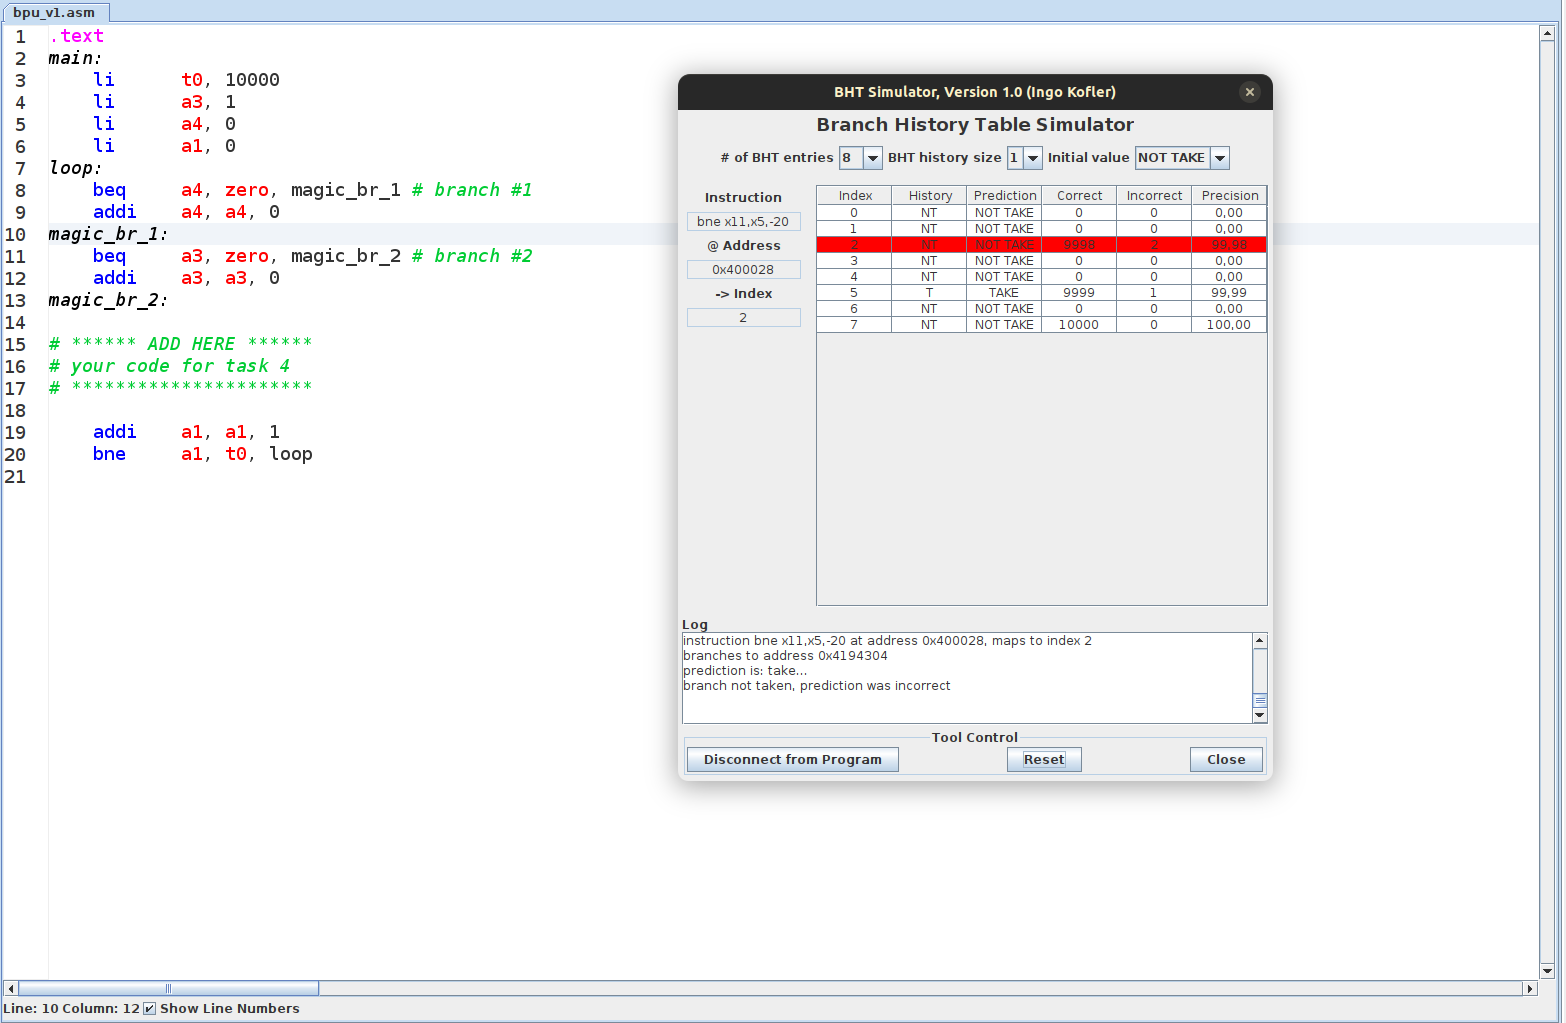
\includegraphics[width=0.9\linewidth]{btb1.png}
    \caption{Рис. \ref{fig:btb1}. Состояние BHT после завершения исходной программы}
    \label{fig:btb1.png}
\end{figure}

Точность предсказания magic\_br\_1 - 100\%

Точность предсказания magic\_br\_2 - 99.99\%

\section*{Пункт 2}

\begin{figure}[h!]
    \centering
    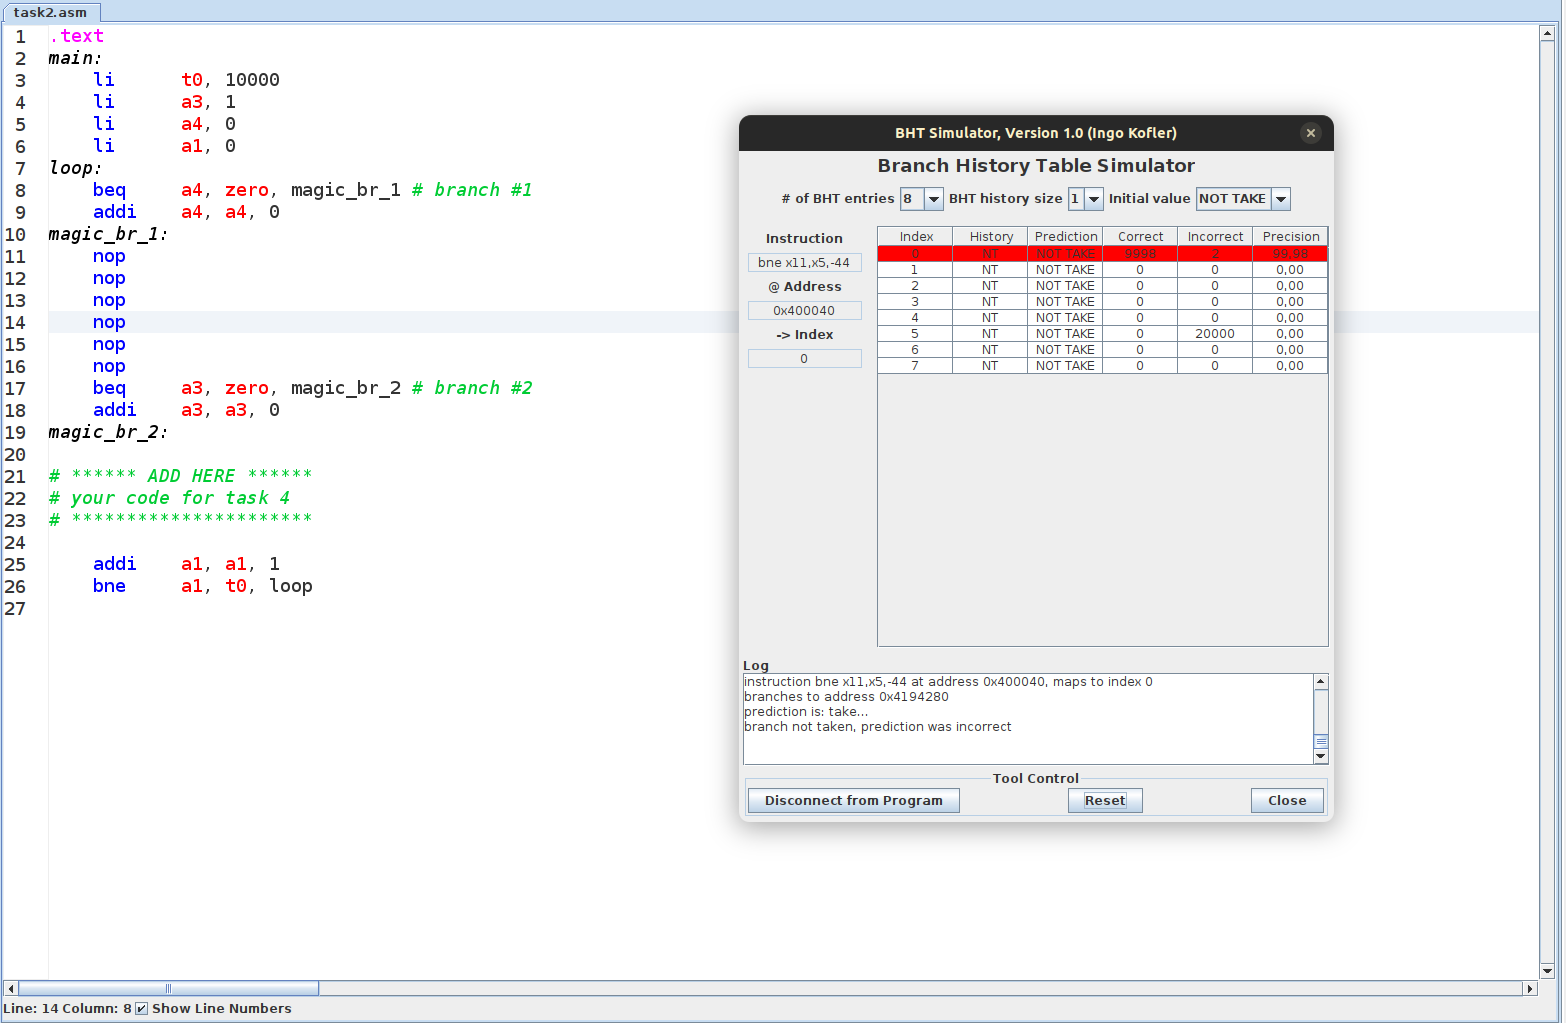
\includegraphics[width=0.9\linewidth]{btb2.png}
    \caption{Рис. \ref{fig:btb2}. Состояние BHT после завершения программы, со вставленными nop}
    \label{fig:btb2}
\end{figure}

Индекс в таблице BHT зависит от адреса, по котором располагается инструкция перехода. Чтобы следующая инструкция перехода использовала индекс предыдущей, между ними должно быть расстояние в количество инструкций, кратное BHT entries. Поэтому добавим 6 nop (так как уже есть инстуркциz addi) после перехода magic\_br\_1. Тогда оба перехода будут попадать на один и тот же индекс в BHT. А так как первый переход всегда TAKEN, то Predication на следующий прыжок будет тоже TAKEN (ожидаем, что раз уж мы TAKEN, то и потом тоже будем). Второй переход всегда NOT TAKEN, поэтому он будет incorrect, и так по кругу. 

\newpage

\section*{Пункт 3}

\begin{figure}[h!]
    \centering
    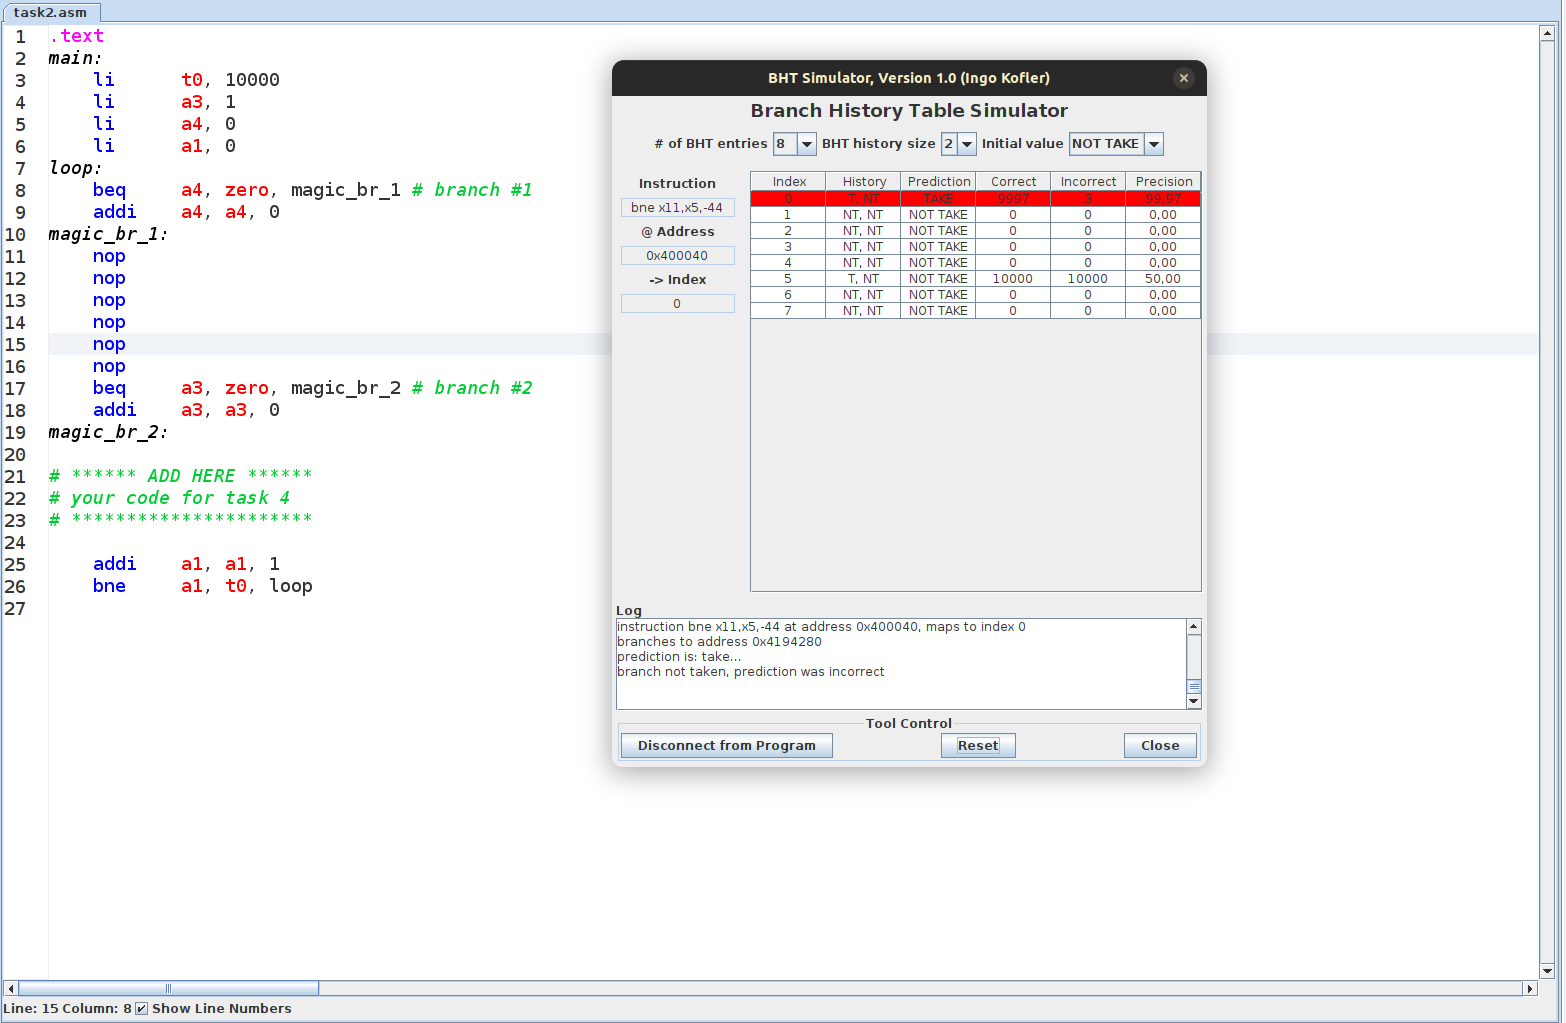
\includegraphics[width=0.9\linewidth]{btb3.png}
    \caption{Рис. \ref{fig:btb3}. Состояние BHT после завершения программы, со вставленными nop, с изменённым настройками}
    \label{fig:btb3}
\end{figure}

Теперь мы поменяли настройки BHT. Prediction основывается не на 1 прошлом прыжке, а сразу на двух. Поэтому чтобы "переубедить" его перейти из крайнего состояния TAKEN / NOT TAKEN в противоположное, требуется 2 incorrect.

На Рис. \ref{fig:state}. показано как мы будем ходить по конечному автомату. Причём incorrect соответствует magic\_br\_1, а correct - magic\_br\_2. А значит

Точность предсказания magic\_br\_1 - 0\%

Точность предсказания magic\_br\_2 - 100\%

\begin{figure}[h!]
    \centering
    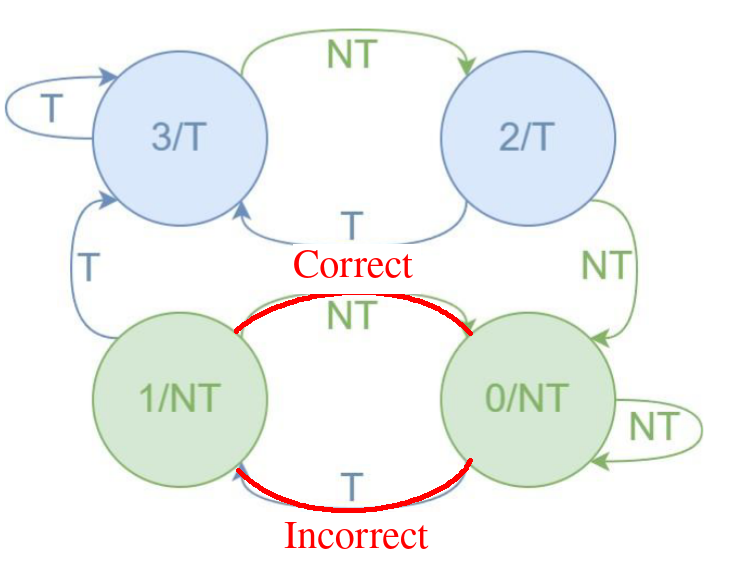
\includegraphics[width=0.5\linewidth]{state1.png}
    \caption{Рис. \ref{fig:state1}. Соответствующий путь по конечному автомату}
    \label{fig:state1}
\end{figure}

\clearpage

\section*{Пункт 4}

\begin{figure}[h!]
    \centering
    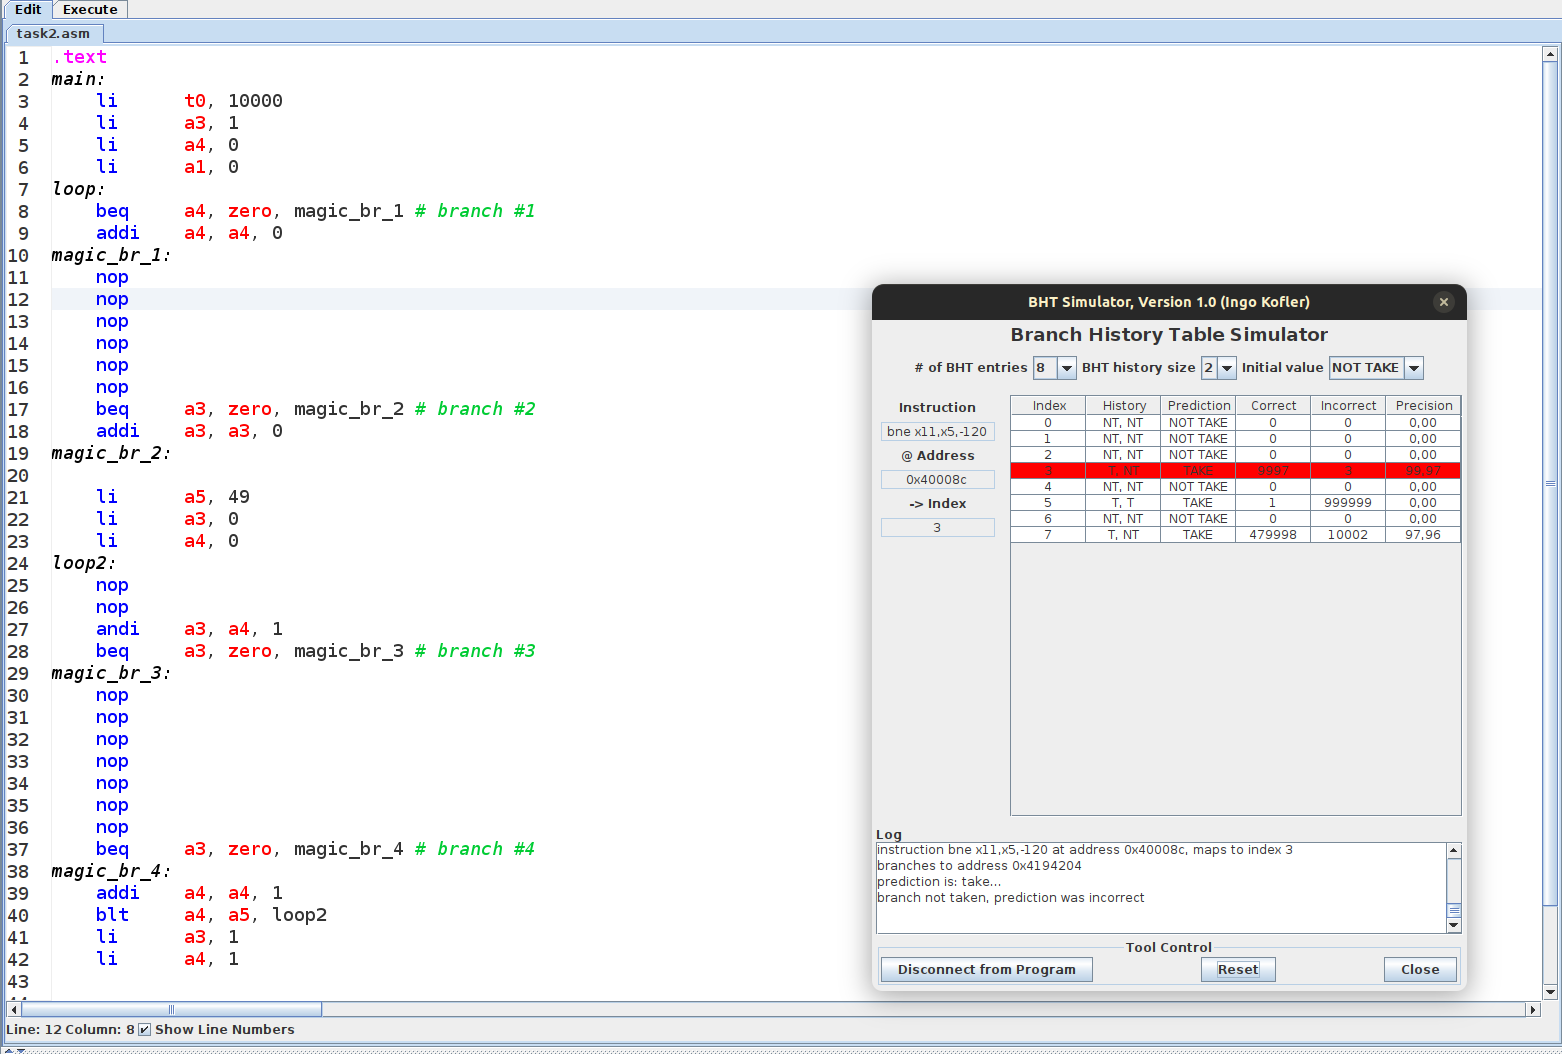
\includegraphics[width=0.9\linewidth]{btb4.png}
    \caption{Рис. \ref{fig:btb4}. Состояние BHT после завершения программы с двумя добавленным beq}
    \label{fig:btb4}
\end{figure}

Нам нужно добавить ещё 2 перехода, чтобы точность предсказания всех четырёх переходов была не больше 0.0001\%. 1 раз у нас точно будет correct на втором переходе, так как мы не можем ничего менять в этой части кода. Значит нам нужно Добиться 999999 incorrect. Если нам нужны все incorrect, то наш путь по состояниям будет как на Рис. \ref{fig:state2}. 

\begin{figure}[h!]
    \centering
    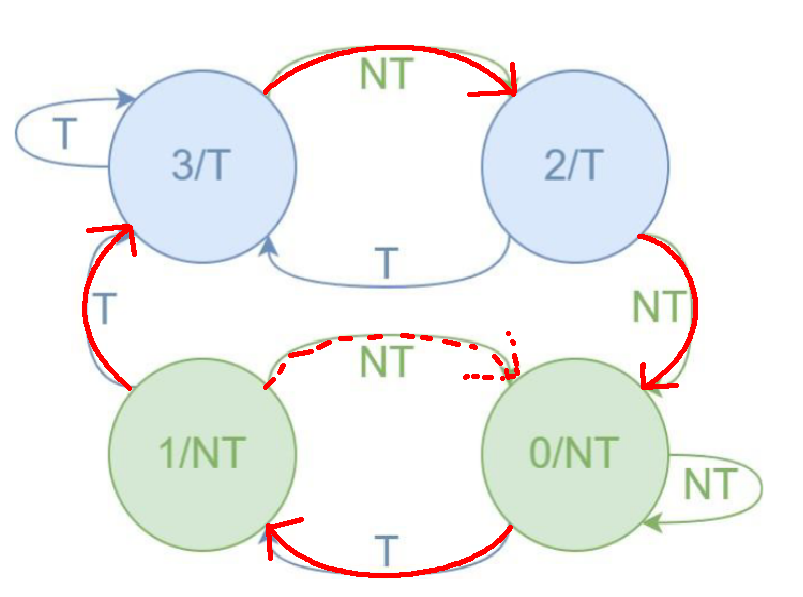
\includegraphics[width=0.4\linewidth]{state2.png}
    \caption{Рис. \ref{fig:state2}. Соответствующий путь по конечному автомату. Пунктиром показан единственный correct переход на magic\_br\_2.}
    \label{fig:state2}
\end{figure}

Напишем цикл, внутри которого будут наши дописанный третий и четвёртый переходы. Если мы всё время получаем incorrect, значит prediction будет чередоваться каждый 2 перехода, то есть в конетксте цикла каждую итерацию. Значит На первой итерации у нас должно быть TAKEN и TAKEN, на второй NOT TAKEN и NOT TAKEN и так далее. Это соответствует чётности счётчика. Будет делать andi счётчика с единичкой и проверять это значение на 0. 

Сделаем количество итераций внутреннего цикла 49, потому что для получения 999999 incorrect нужно $2\cdot10000 + 49\cdot2\cdot10000 = 1000000$ переходов. И нам повезло, ведь если итераций внутреннего цикла нечётное количество, то в начале каждой новой итерации внешнего цикла будет одно и то же состояние BHT, а именно 3/T, поэтому не надо мудрить с чётностью a1, и можно просто после внутреннего цикла выставить a3 и a4 в числа отличные от нуля (в целом a4 можно и не выставлять, потому что он используется как счётчик во внутреннем цикле и точно будет больше 0, но для симметрии). При этом перед входом во внутренний цикл у нас тоже всегда (даже на нулевой итерации) будет одно и то же состояние на каждой итерации, а именно 0/NT, а значит на первой итерации внутреннего цикла третий и четвёртый переходы должны быть TAKEN (соответствует проверке счётчика именно на чётность а не на нечётность).

Ну и конечно, чтобы все наши 4 перехода попадали в один индекс BHT, добавляем nop-ов, чтобы количество инструкций между ними было кратно 8 (BHT entries).

\end{document}